% Created 2025-07-09
% Intended LaTeX compiler: pdflatex
\documentclass[11pt,a4paper]{article}

% ──────────────────────── Paquetes básicos ────────────────────────
\usepackage[utf8]{inputenc}
\usepackage[T1]{fontenc}
\usepackage[english, spanish]{babel}
\usepackage{graphicx}
\usepackage{grffile}
\usepackage{longtable}
\usepackage{wrapfig}
\usepackage{rotating}
\usepackage[normalem]{ulem}
\usepackage{amsmath, amssymb}
\usepackage{textcomp}
\usepackage{capt-of}
\usepackage{tabularx}
\usepackage{lastpage}
\usepackage{enumitem}
\usepackage[table,xcdraw]{xcolor}
\usepackage[left=2.00cm,right=2.50cm,top=2.50cm,bottom=2.50cm]{geometry}
\usepackage{hyperref}

% ──────────────────────── Comandos útiles ────────────────────────
\newcommand*{\autor}[1]{\def\authorname{#1}}
\newcommand*{\titulo}[1]{\def\@title{#1}\def\ttitle{#1}}
\newcommand{\versionActual}{A}
\newcommand{\fechaA}{09/07/2025}
\newcommand{\fechaB}{}
\newcommand{\fechaC}{}
\newcommand{\docCode}{\normalsize RETRO\_GAME-DD versión \versionActual}

\titulo{Videojuego portátil inspirado en consolas retro}      % <─ Cambia si quieres
\autor{Lic. Jezabel Danon}

\usepackage{ifthen}
\newcommand{\fechaActual}{%
  \ifthenelse{\equal{\versionActual}{A}}{\fechaA}{%
    \ifthenelse{\equal{\versionActual}{B}}{\fechaB}{%
      \ifthenelse{\equal{\versionActual}{C}}{\fechaC}{
        N/A
      }}}}

% ──────────────────────── Encabezado / pie ────────────────────────
\usepackage{fancyhdr}
\fancyhf{}
\pagestyle{fancy}
\lhead{
\includegraphics[width=3.5cm]{../Figuras/logoFIUBA.pdf}}
\rhead{\normalsize\textbf{\@title}\\Documento de diseño de software\\\docCode}
\setlength{\headheight}{42pt}
\setlength{\footskip}{25pt}
\cfoot{\normalsize Página \thepage\ de \pageref{LastPage}}
\renewcommand{\headrulewidth}{1pt}
\renewcommand{\footrulewidth}{0.4pt}

% ──────────────────────── Hyperref ────────────────────────
\hypersetup{
  colorlinks=true,
  linkcolor=black,
  urlcolor=blue,
  pdftitle={\@title},
  pdfauthor={\authorname},
  pdflang={es}
}

% ──────────────────────── Documento ────────────────────────
\begin{document}

% ---------- Portada ----------
\begin{titlepage}
  \centering
  
\includegraphics[width=.7\textwidth]{../Figuras/logoFIUBA.pdf}\par
  \vspace{1cm}
  {\Huge\textbf{\ttitle}}\par
  \vspace{1.5cm}
  {\Large\itshape Documento de diseño de software (SDD)\par}
  \vspace{3cm}
  \flushleft
  {\normalsize Autor:}\par
  {\Large \authorname\ (jezabel.danon@gmail.com)}\par
  \vspace{1.5cm}
  {\scshape\LARGE \fechaActual}\par
  {\scshape\LARGE Versión \versionActual}\par
  \vfill
  \centering
  \textit{Basado en el estándar IEEE 1016-2017.}
\end{titlepage}

\clearpage            % fuerza una nueva página real
\pagestyle{fancy}     % activa encabezado y pie desde esta página

\section*{Historial de cambios}
\pagestyle{fancy}     % activa el estilo fancy para el resto
\begin{table}[ht]
\label{tab:registro}
\centering
\begin{tabularx}{\linewidth}{@{}|c|c|X|c|c|@{}}
\hline
\rowcolor[HTML]{C0C0C0} 
Versión & Fecha & \multicolumn{1}{c|}{\cellcolor[HTML]{C0C0C0}Descripción}  & Autor & Revisores     \\ \hline
A   & \fechaA   & Creación del documento     & \authorname     &                        \\ \hline
\end{tabularx}
\end{table}

\pagebreak

\clearpage
\tableofcontents
\clearpage

% ---------- 1 Introducción ----------
\section{Introducción}
\subsection{Propósito}
\begin{enumerate}
  \item Este documento describe el diseño del software para el sistema embebido \textit{\ttitle}. 
  \item Está dirigido a los desarrolladores que se ocupen del análisis, diseño e implementación del software, así como también a quienes desarrollen el testing, validaciones y/o verificaciones del mismo.
\end{enumerate}

\subsection{Ámbito}
\begin{enumerate}
  \item El sistema está compuesto por un dispositivo embebido portátil que integra entradas físicas (botones, joystick, acelerómetro), salidas audiovisuales (pantalla, parlante, vibración) y una unidad de procesamiento encargada de coordinar la ejecución de un demo de juego simple.
  \item El presente diseño de software abarca los módulos encargados de:
  \begin{itemize}
    \item Control de entrada/salida digital y analógica.
    \item Gestión del flujo del juego.
    \item Renderizado gráfico en pantalla.
    \item Generación de audio y control de vibración.
    \item Manejo de estados internos y lógica de juego.
  \end{itemize}
  \item Este documento se enfoca exclusivamente en la descripción estructural y funcional del software embebido. No se incluyen aspectos de diseño físico, elección final de componentes electrónicos ni pruebas de verificación, los cuales son abordados en documentos específicos (como las especificaciones de hardware).
  \item El diseño cubre las capas de abstracción de hardware (drivers), lógica de control del juego, gestión de recursos gráficos y sonoros, así como el manejo de entradas y salidas del sistema. 
  \item Quedan fuera de este documento los detalles de bajo nivel sobre protocolos específicos de comunicación (como I\textsuperscript{2}C o SPI), que se encuentran documentados en los manuales de componentes o en la especificación de hardware.
  \item Tampoco se incluyen aspectos de programación de la interfaz de usuario en cuanto a estilo o experiencia visual final, los cuales podrán ser definidos en una etapa posterior del desarrollo.
\end{enumerate}

\subsection{Definiciones y acrónimos}
  \begin{enumerate}
    \item IEEE: Instituto de Ingenieros Eléctricos y Electrónicos.
    \item ERS: Especificación de Requisitos de Software.
    \item RTOS: Sistema Operativo de Tiempo Real (Real Time Operating System).
    \item CMSIS: Arm's Common Microcontroller Software Interface Standard. Se compone por un conjunto de APIS, componentes de software, herramientas y flujos de trabajo provisto por el desarrollador de la arquitectura del microcontrolador a utilizar.
    \item HAL: Hardware Abstraction Layer. Conjunto de bibliotecas de software provistas por STMicroelectronics para simplificar la interacción con el hardware de microcontroladores STM32.
    \item UI: Interfaz de usuario (User Interface).
    \item UART: Universal Asynchronous Receiver/Transmitter. 
    \item I2C: Inter-Integrated Circuit.
    \item SPI: Serial Peripheral Interface.
    \item ADC: Analogic to Digital Converter.
    \item PWM: Pulse Width Modulation.
    \item GPIO: General-purpose Input/Output.
    \item ST-Link: programador y depurador integrado en placas STM32.
    \item N/A: No Aplica.
  \end{enumerate}

\subsection{Referencias}

\begin{enumerate}
  \item \href{https://drive.google.com/file/d/1C3vEYR8wME6EzlZVVC-gT2u86dwnoZA-/view?usp=sharing}{Plan de proyecto del trabajo práctico final} para la \textit{Carrera de Especialización en Sistemas Embebidos} (RETRO\_GAME-PP-v5). 
  \item Especificaciones de requisitos de software: RETRO\_GAME-RS-vA.
  \item Especificaciones de requisitos de hardware: RETRO\_GAME-RH-vA.
  \item Especificaciones de casos de uso: RETRO\_GAME-CU-vA.
  \item Documento de arquitectura: RETRO\_GAME-AR-vA.
\end{enumerate}

% ---------- 2 Resumen de la arquitectura ----------
\section{Resumen de la arquitectura}
\begin{enumerate}
  \item El sistema software para el sistema embebido \textit{\ttitle} se basa en una arquitectura modular y estratificada, descrita en profundidad en el documento de arquitectura \textit{RETRO\_GAME-AR}. 

  \item El software se organiza en tres capas principales:

  \begin{itemize}
    \item \textbf{Capa de drivers}: incluye los controladores de bajo nivel responsables de inicializar y acceder a los periféricos físicos (pantalla TFT por SPI, audio por PWM, EEPROM por I\textsuperscript{2}C, entradas físicas por GPIO/ADC y temporizadores). 

    \item \textbf{Lógica del sistema}: contiene los servicios de propósito general como el gestor de estados del sistema, el manejador de eventos, el cargador de recursos gráficos y sonoros, el subsistema de persistencia y el motor de interfaz de usuario. Esta capa actúa como intermediaria entre los drivers y la lógica del juego, manteniendo la consistencia y coordinando flujos.

    \item \textbf{Lógica del juego}: implementa el comportamiento específico del gameplay. Incluye su propia máquina de estados, el motor de renderizado de escenas y la lógica que interpreta eventos de entrada como acciones dentro del juego.

  \end{itemize}

  \item El sistema corre sobre un RTOS de tipo cooperativo con planificación por prioridad fija. Las tareas concurrentes están organizadas por funcionalidad (drivers, UI, lógica del juego) y se comunican mediante colas, semáforos y señales. La arquitectura favorece un desacoplamiento fuerte entre capas, facilitando el testeo modular y la reutilización de servicios comunes.

  \item Este documento de diseño detallado expande la descripción de cada uno de los módulos presentados en esta arquitectura, definiendo su comportamiento interno, sus estructuras de datos y sus interfaces.

\end{enumerate}

% ---------- 3 Diseño detallado de módulos y servicios ----------
\section{Diseño detallado de módulos y servicios}

A continuación se presenta el listado de componentes por capa junto a una breve descripción de sus responsabilidades.

\begin{longtable}{|p{2cm}|l|p{3cm}|p{6.5cm}|}
% \caption{Componentes del sistema y responsabilidades}\\
\hline
\textbf{Capa} & \textbf{Servicio } & \textbf{Nombre} & \textbf{Responsabilidad principal} \\
\hline
\endfirsthead
\cline{1-1}
\endfoot

\hline
\textbf{Capa} & \textbf{Servicio } & \textbf{Nombre} & \textbf{Responsabilidad principal} \\
\hline
\endhead
\cline{1-1}
\endlastfoot

\textbf{Drivers} & \texttt{AccelDrv} & Driver de acelerómetro & Lectura por I\textsuperscript{2}C \\
\cline{2-4}
& \texttt{EEPROMDrv} & Driver de memoria EEPROM & Lectura y escritura por SPI \\
\cline{2-4}
& \texttt{ScreenDrv} & Driver de pantalla & Control ST7735, ventana activa, transferencia de píxeles por SPI/DMA \\
\cline{2-4}
& \texttt{AudioDrv} & Driver de audio & Reproducción de efectos de sonido mediante modulación por ancho de pulso (PWM) \\
\cline{2-4}
& \texttt{HapticDrv} & Driver de vibración & Comunicación con DRV2605L por I\textsuperscript{2}C, ejecución de patrones \\
\cline{2-4}
& \texttt{UARTDrv} & Driver de UART & Comunicación USART2 (DMA); base para consola de debug \\
\cline{2-4}
& \texttt{InputDrv} & Driver de entradas & Lectura de botones (EXTI) y joystick (ADC DMA), empaqueta eventos crudos \\
\cline{2-4}
& \texttt{TimerDrv} & Driver de timers & Generación de interrupciones de tiempo \\
\hline

\textbf{Lógica del sistema} & \texttt{BootMgr} & Gestor de arranque & Inicializa drivers, crea tareas FreeRTOS, transfiere a menú principal \\
\cline{2-4}
& \texttt{ResLoader} & Cargador de recursos & Carga de recursos (imágenes, sonidos) en RAM desde memoria externa \\
\cline{2-4}
& \texttt{ConfigPersist} & Configuración y persistencia & Guarda/carga snapshot de juego; verificación de partida guardada \\
\cline{2-4}
& \texttt{EventDispatcher} & Despachador de eventos & Normaliza entradas y publica eventos a tareas superiores; redistribución de mensajes entre componentes \\
\cline{2-4}
& \texttt{UIController} & Gestor de interfaz de usuario & Gestión de la UI en estados no interactivos del juego \\
\cline{2-4}
& \texttt{GraphEngine} & Motor gráfico & Renderizado gráfico, gestión de buffers de pantalla \\
\cline{2-4}
& \texttt{AudioPlayer} & Reproductor de sonido & Mezcla y reproduce música o efectos \\
\cline{2-4}
& \texttt{HapticEngine} & Motor háptico & Gestión de la activación de patrones de vibración \\
\cline{2-4}
& \texttt{LogSink} & Debug y logs & Gestión de comunicaciones por UART y trazas de depuración \\
\cline{2-4}
& \texttt{SysMng} & Gestión de estados del sistema & Implementación de máquina de estados principal del sistema,
gestión de transiciones (\texttt{SYS\_SPLASH, SYS\_MAIN\_MENU, SYS\_IN\_GAME, SYS\_PAUSED}) \\
\hline

\textbf{Lógica del juego} & \texttt{GameMng} & Gestión de estado del juego & Control del bucle de juego, construcción del modelo
gráfico; implementación de los estados internos del juego (\texttt{GME\_RUNNING, GME\_FROZEN, GME\_STOPPED)} \\
\cline{2-4}
& \texttt{RenderEngine} & Motor de renderizado & Generación del contenido visual del juego para cada cuadro; coordinación con servicios de generación de salidas \\
\cline{2-4}
& \texttt{InputHandler} & Gestión de entradas & Traducción de eventos normalizados a acciones de gameplay \\
\cline{2-4}
\end{longtable}


% \subsection{Estructura de carpetas del código}

%-------------------------------------- Capa Drivers
\subsection{Drivers}

\subsubsection{\texttt{AccelDrv} — Driver de acelerómetro}
\paragraph{Resumen:} Controla la comunicación con el sensor MPU-6500 a través del bus I\textsuperscript{2}C. Permite obtener valores de aceleración crudos en los tres ejes para su posterior uso en lógica de juego o UI.
\paragraph{Notas adicionales:}
\begin{itemize}
  \item Se debe configurar la dirección de I2C y registrar la interrupción de "data ready".
  \item Solo se utilizará el acelerómetro (y solo 2 ejes); se puede deshabilitar el giroscopio para ahorrar consumo.
  \item Requiere setup inicial del registro PWR\_MGMT y escala de sensibilidad.
  \item Retorna: datos x DMA ({ACC\_X, ACC\_Y}) evento para EventDispatcher (DRV\_OK, DRV\_ERR)
\end{itemize}

\subsubsection{\texttt{EEPROMDrv} — Driver de memoria EEPROM}
\paragraph{Resumen:} Brinda una interfaz para operaciones de lectura y escritura en la memoria EEPROM SPI 25LC256, utilizada para snapshots y configuraciones.
\paragraph{Notas adicionales:}
\begin{itemize}
  \item Debe controlar el pin \texttt{CS} manualmente.
  \item Implementar verificación de página y latencia de escritura.
  \item Usar checksum CRC para validar snapshots.
  \item Recibe: [data,] direccion
  \item Retorna [data,] ok/fail, evento para EventDispatcher (DRV\_OK, DRV\_ERR, info de guardado y carga)
\end{itemize}

\subsubsection{\texttt{ScreenDrv} — Driver de pantalla}
\paragraph{Resumen:} Controla la pantalla TFT de 1.8" con controlador ST7735R mediante SPI. Permite enviar bloques de píxeles desde un búfer de imagen RAM.
\paragraph{Notas adicionales:}
\begin{itemize}
  \item Usa DMA para transferencias rápidas de píxeles.
  \item Es mayormente el driver TFT\_ST7735 ya desarrollado.
  \item Considerar la implementación de "ventana activa" para actualizar solo regiones.
  \item Retorna: evento para EventDispatcher  (DRV\_OK, DRV\_ERR, alguna info de renderizado o flush??)
\end{itemize}

\subsubsection{\texttt{AudioDrv} — Driver de audio}
\paragraph{Resumen:} Genera salida de audio mediante modulación PWM y amplificador externo (LM386). Se alimenta con datos desde el \texttt{AudioPlayer}.
\paragraph{Notas adicionales:}
\begin{itemize}
  \item Usar PWM de alta frecuencia (al menos 20 kHz). % con DMA circular solo si es música constante.
  \item Controlar el volumen mediante ajuste de duty o por hardware.
  \item Entradas: frecuencia fija o muestras PCM, duración (\{*pcm, durtionMs\})
  \item Retorna evento para EventDispatcher  (DRV\_OK, DRV\_ERR, info de envio de datos)
  % \item Silenciamiento rápido en pausa o errores.
\end{itemize}

\subsubsection{\texttt{HapticDrv} — Driver de vibración}
\paragraph{Resumen:} Controla el módulo DRV2605L por I\textsuperscript{2}C para generar patrones de vibración con motor ERM.
\paragraph{Notas adicionales:}
\begin{itemize}
  \item El DRV2605L tiene biblioteca interna de patrones ROM.
  \item Requiere escritura de patrón y activación del disparo.
  \item Considerar cola de vibraciones para evitar pérdidas.
  \item Entradas: id del patrón de vibración a reproducir.
  \item Retorna evento para EventDispatcher  (DRV\_OK, DRV\_ERR, info de envio de datos)
\end{itemize}

\subsubsection{\texttt{UARTDrv} — Driver de UART}
\paragraph{Resumen:} Maneja la comunicación serie con la PC a través de USART2, principalmente para logging y comandos de consola.
\paragraph{Notas adicionales:}
\begin{itemize}
  \item Configurar USART2 con DMA para recepción continua.
  \item Reconocimiento de comando de on/off.
  \item Se conecta vía ST-Link como puerto virtual.
  \item Retorna eventos para EventDispatcher  (DRV\_OK, DRV\_ERR, CMD\_LOGON, CMD\_LOGOFF)
\end{itemize}

\subsubsection{\texttt{InputDrv} — Driver de entradas}
\paragraph{Resumen:} Lee botones físicos mediante interrupciones (GPIO/EXTI) y joystick analógico mediante ADC. Entrega eventos crudos al despachador.
\paragraph{Notas adicionales:}
\begin{itemize}
  \item Debounce por software.
  \item ADC con conversión continua + DMA para eje X/Y (??)
  \item Agrupar estado en estructura con bitmask de botones + valores analógicos.
  \item Retorna eventos para EventDispatcher  (DRV\_OK, DRV\_ERR, BTN\_X\_PRESS, {JY\_X, JY\_Y})
\end{itemize}

\subsubsection{\texttt{TimerDrv} — Driver de temporizadores}
\paragraph{Resumen:} Proporciona temporización periódica (ej. tick de frame) mediante timers de hardware. Puede generar interrupciones o callbacks.
\paragraph{Notas adicionales:}
\begin{itemize}
  \item Base para lógica temporal en el juego y animaciones.
  \item Se usará probablemente TIM2 o TIM3.
  \item Considerar usar HAL Timer + callbacks con prioridad baja.
\end{itemize}

%-------------------------------------- Capa Sistema
\subsection{Componentes de sistema }

\subsubsection{\texttt{BootMgr} — Gestor de arranque}
\paragraph{Resumen:} Se ejecuta al inicio del sistema tras el bootloader. Se encarga de inicializar los servicios básicos, crear las tareas de FreeRTOS y mostrar la pantalla inicial (splash).
\paragraph{Notas adicionales:}
\begin{itemize}
  \item Debería inicializar los drivers y gestionar que todos funciones OK.
  \item Llamar a ConfigPersist para que revise partida guardada para renderizar el menú ppal.
  \item Crea colas, inicializa módulos y transfiere el control a \texttt{SysMng} (\texttt{SYS\_READY}).
  \item Puede verificar integridad del sistema o mostrar fallos iniciales.
\end{itemize}

\subsubsection{\texttt{ResLoader} — Cargador de recursos}
\paragraph{Resumen:} Permite leer recursos binarios como sprites, fuentes o jingles desde EEPROM externa o memoria Flash, y ponerlos en RAM para uso por los motores gráficos o de audio.
\paragraph{Notas adicionales:}
\begin{itemize}
  \item Solo lectura. Desacoplado del guardado.
  \item Puede usar índice predefinido o direcciones fijas:
  \begin{itemize}
    \item mapa de la memoria EEPROM, secciones predefinidas para assets, profile/configs, juego
    \item tabla de id-location para assets predefinidos/precargados en memoria
  \end{itemize}
  \item Debe notificar cuando el recurso esté listo vía evento.
  \item Entradas: id del asset a cargar (unsigned int).
  \item Retorna eventos para EventDispatcher (RES\_READY) y asset serializado
\end{itemize}

\subsubsection{\texttt{ConfigPersist} — Persistencia y configuración}
\paragraph{Resumen:} Gestiona el guardado y restauración del estado del juego (snapshot) y configuraciones persistentes. Se comunica con \texttt{EEPROMDrv}.
\paragraph{Notas adicionales:}
\begin{itemize}
  \item Es responsable del mapeo de direcciones y formato de snapshot.
  \item Requiere validación con checksum/CRC.
  \item Debería poder distinguir entre guardado válido y vacío.
  \item Mapa de la memoria EEPROM, secciones predefinidas para assets, profile/configs, juego
  \item Regiones de memoria para los snapshots y flag HAS\_SAVE .
  \item Generacion del campo flag HAS\_SAVE y guardado en region config (acceso mas simple que el snap).
  \item Retorno de eventos al EventDispatcher (CFG\_SAVE\_DONE, CFG\_SAVE\_ERR, CFG\_HAS\_SAVE)
\end{itemize}

\subsubsection{\texttt{EventDispatcher} — Despachador de eventos}
\paragraph{Resumen:} Recibe eventos crudos desde \texttt{InputDrv}, los normaliza (antirrebote, umbral, zona muerta) y los distribuye a tareas lógicas superiores mediante colas o flags.
\paragraph{Notas adicionales:}
\begin{itemize}
  \item Es el único punto entre entradas físicas y lógica del sistema/juego.
  \item Convierte joystick a ejes discretos (ej. izquierda, centro, derecha) y boton X a BTN\_START. 
  \item Procesamiento de inclinación (si es necesario)
  \item Guarda la bandera traceEnabled. Si true, duplica cada mensaje que rutea hacia queueLogSink.
  \item Todos los eventos deben pasar por aca para redistribuir a log.
  \item Tabla origen/evento --> destinatario
\end{itemize}

\subsubsection{\texttt{UIController} — Interfaz de usuario}
\paragraph{Resumen:} Controla pantallas como menú principal, pausa, confirmaciones o mensajes fuera del gameplay. Interpreta entradas y publica acciones internas.
\paragraph{Notas adicionales:}
\begin{itemize}
  \item Dibuja menus con LVGL. 
  \begin{itemize}
    \item Si pongo los lv\_port en GraphEngine, entonces UIController estaria tecnicamente enviado la data al GraphEngine
    \item Envia lista de objetos gráficos (struct: drawList\{\})) a GraphEngine (mas o meno lo hace la libreria LVGL)
  \end{itemize}
  \item Integración con sonido y vibración (??)
  \begin{itemize}
    \item datos para reproducción de audio (audioCue \{id, duration\}).
    \item datos para generación de vibración (hapticCue enum: SEND\_PATTERN\_1, SEND\_PATTERN\_2).
  \end{itemize}
\end{itemize}

\subsubsection{\texttt{GraphEngine} — Motor gráfico}
\paragraph{Resumen:} Proporciona primitivas 2D para dibujar en pantalla: sprites, textos, rectángulos. Coordina el doble búfer y compone la display-list para \texttt{ScreenDrv}.
\paragraph{Notas adicionales:}
\begin{itemize}
  \item Seria un wrapper de las cosas que voy a usar de LVGL
  \item Si pongo los lv\_port en GraphEngine, entonces UIController estaria tecnicamente enviado la data al GraphEngine
  \item Aca hay que armar todas las primitivas que podrian usar LVGL por abajo para renderizar los graficos del juego a partir de la RenderList o drawList (Objetos lógicos: {layer, spriteID, posX, posY})
  \item Ideal tener una cola o display-list reutilizable.
  \item Ofrece API común a UI y juego.
  \item Prioridad baja en renderizado; puede reducir FPS en pausa.
\end{itemize}

\subsubsection{\texttt{AudioPlayer} — Motor de audio}
\paragraph{Resumen:} Mezcla efectos de sonido y música, y los entrega a \texttt{AudioDrv}. Permite silenciar, repetir, interrumpir o atenuar sonidos.
\paragraph{Notas adicionales:}
\begin{itemize}
  \item Controla el buffer circular y su tasa.
  \item Soporta volúmenes diferenciados.
  \item Puede tener canal reservado para jingles o música de fondo.
\end{itemize}

\subsubsection{\texttt{HapticEngine} — Motor háptico}
\paragraph{Resumen:} Programa el driver DRV2605L con patrones de vibración en respuesta a eventos del sistema o juego.
\paragraph{Notas adicionales:}
\begin{itemize}
  \item Puede implementar una cola de eventos con prioridad.
  \item Compatible con patrones integrados del DRV2605L.
  \item Deshabilitado automáticamente durante muting o en pausa.
\end{itemize}

\subsubsection{\texttt{LogSink} — Debug y logs}
\paragraph{Resumen:} Canaliza mensajes del sistema o juego hacia la UART, para ser interpretados por consola o herramientas externas.
\paragraph{Notas adicionales:}
\begin{itemize}
  \item Usa \texttt{UARTDrv} como backend.
  \item Incluye flag para activar/desactivar salida.
  \item Posibilidad de implementar comandos de texto para debug.
\end{itemize}

\subsubsection{\texttt{SysMng} — Gestión de estados del sistema}
\paragraph{Resumen:} Implementa la FSM principal del sistema embebido. Administra transiciones globales como encendido, menú principal, pausa y juego activo.
\paragraph{Notas adicionales:}
\begin{itemize}
  \item Encapsula los modos \texttt{SYS\_SPLASH}, \texttt{SYS\_MENU}, \texttt{SYS\_IN\_GAME}, \texttt{SYS\_PAUSED}.
  \item Activa/desactiva módulos según contexto.
  \item Dispara los estados de juego al iniciar o salir.
\end{itemize}

\subsection{Componentes del juego}

\subsubsection{\texttt{GameMng} — Gestor de estado del juego}
\paragraph{Resumen:} Controla el bucle principal del gameplay. Define y administra los estados internos del juego como ejecución activa, pausa y finalización.
\paragraph{Notas adicionales:}
\begin{itemize}
  \item Implementa una FSM propia independiente de \texttt{SysMng}.
  \item Responsable de invocar a \texttt{UpdateEngine}, \texttt{RenderEngine} y servicios de salida.
  \item Emite eventos como \texttt{PLAY\_SFX}, \texttt{VIBRATE\_HIT}, \texttt{EXIT\_TO\_MENU}.
  \item Debe poder congelar el juego sin perder el estado (ej. en pausa o guardado).
  \item Genera gameModel que encapsule subt-structs: Player, World 
  \begin{itemize}
    \item Contiene todo lo que hace falta — cada frame — para actualizar la lógica y dibujar la escena
    \item Lo que no puede calcularse del gameModel a partir de otras variables, es lo que se va a guardar en el snapshot
    \item 
  \end{itemize}
  \item Genera gameSignal[]: vector / cola de “hechos relevantes”
  % \begin{itemize}
  %   \item Comparando estado actual vs. anterior:
  %   \item  Velocidad menor a stall_thr -> SIG\_STALL\_WARN
  %   \item  Way-point alcanzado -> SIG\_WP\_REACHED
  % \end{itemize}
\end{itemize}

% GameModel                 // ≈ 24 bytes
% ┌──────────────────────────┐
% │ nav_x_cm      int32  ↳ Física                // posición en el mapa (cm)
% │ nav_y_cm      int32  ↳ Física
% │ heading_deg   int16  ↳ Física (0-359)        // “rumbo” usado para elegir horizonte
% │ speed_cm_s    int16  ↳ Física                // avance longitudinal
% │
% │ cam_tilt      int8   ↳ Input                 // vista arriba/abajo   –100…+100 %
% │ cam_pan       int8   ↳ Input                 // vista izquierda/dcha –100…+100 %
% │
% │ frame_ms      uint32 ↳ Tick global           // cronómetro de juego
% └──────────────────────────┘

% typedef struct {
%     int32_t nav_x_cm;
%     int32_t nav_y_cm;
%     int16_t heading_deg;
%     int16_t speed_cm_s;
%     int8_t  cam_tilt;      // -100…+100 %
%     int8_t  cam_pan;       // -100…+100 % 
%     uint32_t frame_ms;     // cronómetro runtime
% } GameModel;
% ojo!! (la camara no se mueve individualmente ya que se encuentra "fija" dentro de la cabina del piloto y la unica forma que cambie el enfoque es "moviendo la nave", cuyos movimientos serian acelerar, desacelerar, yaw o giro derecha/izq, aleteo o roll derecha/izq, cabeceo o pitch up/down)


% typedef struct {
%     int32_t nav_x_cm;
%     int32_t nav_y_cm;
%     int16_t heading_deg;
%     int16_t speed_cm_s;
%     uint32_t game_time_ms;   // “tiempo de vuelo” acumulado
%     uint8_t  version;        // para compatibilidad futura
%     uint8_t  crc;            // CRC-8 del bloque
% } SaveState;

% SaveState s = {
%     .nav_x_cm   = model.nav_x_cm,
%     .nav_y_cm   = model.nav_y_cm,
%     .heading_deg= model.heading_deg,
%     .speed_cm_s = model.speed_cm_s,
%     .game_time_ms += elapsed_ms_since_last_save,
%     .version = 1
% };
% s.crc = crc8(&s, sizeof(s)-1);
% asset_store(SAVE_SLOT, &s, sizeof s, NULL);

% typedef enum { SIG_STALL_WARN, SIG_OVERSPEED, SIG_WP_REACHED } GameSignalID;

% typedef struct {
%     GameSignalID id;
%     uint32_t     param;     // opcional (p.ej. idx del way-point)
% } GameSignal;


\subsubsection{\texttt{RenderEngine} — Motor de renderizado del juego}
\paragraph{Resumen:} Construye por cada cuadro la lista de elementos visuales (sprites, textos) que serán enviados al motor gráfico. Define qué se ve en pantalla en función del estado del juego.
\paragraph{Notas adicionales:}
\begin{itemize}
  \item Responsable de composición visual: fondo, entidades, HUD.
  \item Define capas de render (orden de dibujo).
  \item Coordina con \texttt{GraphEngine} para emitir comandos gráficos.
  \item Puede incluir un modo debug visual.
  \item transformacion gameSignal: Tabla de mapeo:
  \begin{itemize}
    \item SIG\_STALL\_WARN → {audio=BEEP1, haptic=TICK}
    \item SIG\_WP\_REACHED → {audio=CHIME, haptic=BUZZ}
  \end{itemize}
\end{itemize}

\subsubsection{\texttt{InputHandler} — Procesador de entradas del juego}
\paragraph{Resumen:} Recibe eventos de entrada desde \texttt{EventDispatcher} y los traduce a acciones dentro del juego, como mover la nave o disparar.
\paragraph{Notas adicionales:}
\begin{itemize}
  \item Ejecuta lógica específica de controles (reglas por juego).
  \item Filtra eventos duplicados o irrelevantes según contexto.
  \item Idealmente desacoplado del hardware y del tipo exacto de entrada.
  \item Puede incluir combinaciones o combos (ej. doble click).
\end{itemize}


\section{Diagramas estáticos relevantes}
\subsection{Relaciones entre módulos}
\subsection{Organización de tareas en FreeRTOS}

% ---------- 5 Modelos dinámicos ----------
\section{Modelos dinámicos}
\subsection{Statecharts}
\begin{figure}[htb]
\centering 
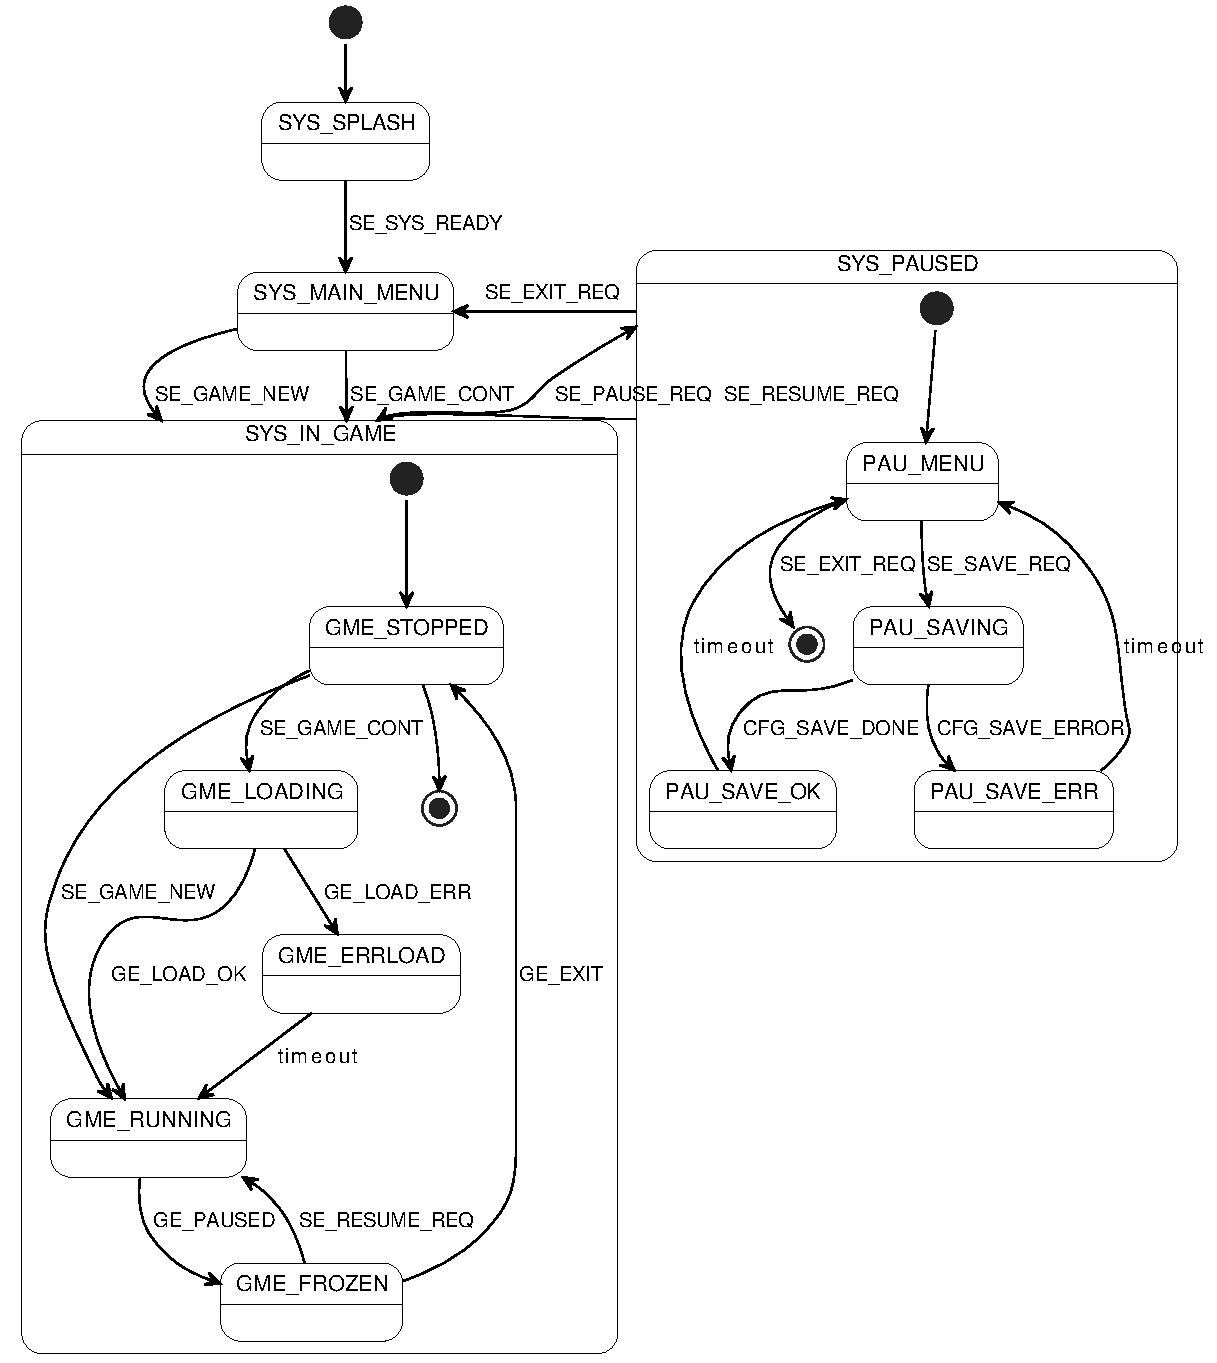
\includegraphics[width=.85\textwidth]{../Figuras/statechart.pdf}
\caption{Diagrama de estados del sistema.}
\label{fig:diagEstados}
\end{figure}

% @startuml
% !pragma layout smetana
% '!pragma layout
% top to bottom direction

% 'skinparam linetype ortho
% skinparam arrow {
%   Color Black
%   Thickness 1
% }
% skinparam state {
%   BackgroundColor #fefefe
%   BorderColor Black
%   ArrowColor Black
% }


% [*] --> SYS_SPLASH
% SYS_SPLASH --> SYS_MAIN_MENU : SE_SYS_READY
% SYS_MAIN_MENU --> SYS_IN_GAME : SE_GAME_NEW
% SYS_MAIN_MENU --> SYS_IN_GAME : SE_GAME_CONT
% SYS_IN_GAME --> SYS_PAUSED : SE_PAUSE_REQ
% SYS_PAUSED --> SYS_IN_GAME : SE_RESUME_REQ
% SYS_PAUSED --> SYS_MAIN_MENU : SE_EXIT_REQ

% state SYS_PAUSED {
%   [*] --> PAU_MENU
%   PAU_MENU --> PAU_SAVING : SE_SAVE_REQ
%   PAU_SAVING --> PAU_SAVE_OK : CFG_SAVE_DONE
%   PAU_SAVE_OK --> PAU_MENU : timeout
%   PAU_SAVING --> PAU_SAVE_ERR : CFG_SAVE_ERROR
%   PAU_SAVE_ERR --> PAU_MENU : timeout
%   PAU_MENU --> [*] : SE_EXIT_REQ
% }

% state SYS_IN_GAME {
%   [*] --> GME_STOPPED
%   GME_STOPPED --> GME_RUNNING : SE_GAME_NEW
%   GME_STOPPED --> GME_LOADING : SE_GAME_CONT
%   GME_LOADING --> GME_RUNNING : GE_LOAD_OK
%   GME_LOADING --> GME_ERRLOAD : GE_LOAD_ERR
%   GME_ERRLOAD --> GME_RUNNING : timeout
%   GME_RUNNING --> GME_FROZEN : GE_PAUSED
%   GME_FROZEN --> GME_RUNNING : SE_RESUME_REQ
%   GME_FROZEN --> GME_STOPPED : GE_EXIT
%   GME_STOPPED --> [*]
% }
% @enduml


\subsection{Diagrama de secuencia 1 - Encendido hasta menú}
% \begin{center}
% %   \includegraphics[width=.9\linewidth]{Figuras/seq_boot_to_menu.pdf}
% \end{center}
Descripción narrativa de cada paso.

\subsection{Diagrama de secuencia 2 - Pausa y opciones}
% \begin{center}
%   \includegraphics[width=.9\linewidth]{Figuras/seq_pause_menu.pdf}
% \end{center}

% ---------- 6 Asignación a tareas y concurrencia ----------
\section{Aspectos de sincronización y concurrencia}
\subsection{Mapa de tareas FreeRTOS}
Tabla con tareas, prioridad, stack, frecuencia.

\subsection{Sincronización y comunicación}
Colas, semáforos, exclusiones mutuas usadas.


% ---------- 7 Aspectos de datos ----------
\section{Modelo de datos}
\subsection{Estructuras persistentes}
Formato del snapshot de partida, layout EEPROM, checksum.

\subsection{Estructuras en RAM}
Buffers de audio, frame buffer, colas de eventos.
% \section{Estructuras de datos clave}
\subsection{Datos en EEPROM}
\subsection{Buffers y estructuras temporales en RAM}

% ---------- 8 Manejo de errores y registro (logging) ----------
\section{Manejo de errores y logs}
Política de códigos de error, niveles de log, rutas de fallos críticos.

\subsection{códigos de error definidos}
\subsection{Ruta de logs por UART}



% ---------- Apéndices ----------
\appendix
\section{Apéndice A - Glosario completo de servicios}
Tabla resumen: Nombre, capa, descripción de 1 línea.

\section{Apéndice B - Diagramas adicionales}
Coloca aquí otros diagramas UML o listas de mensajes.

\end{document}
